\documentclass{resume}

%!TEX program  = xelatex
%%%%%%%%%%%%%%%%%%%%%%%%%%%%%%%%%%%%%%%%%%%%
%                                          %
%  需要的图标请参考文件中的图标包.pdf自行添加   %
%                                          %
%%%%%%%%%%%%%%%%%%%%%%%%%%%%%%%%%%%%%%%%%%%%
\begin{document}


\huge \CJKfamily{heiti} 个人简历\hfill CURRICULUM VITAE
\vspace{10pt}

\begin{minipage}{0.8\textwidth}
	\Large \CJKfamily{heiti} 艾萨克$\cdot$牛顿
	\small 1643.01.04—1727.03.31\\
	\vspace{3pt}
	
	\hspace{0em}
	\begin{tabular}{m{3pt}<{\centering}m{0.5\textwidth}<{\raggedright}m{3pt}<{\centering}m{0.5\textwidth}<{\raggedright}}
	\faMapMarker*  &籍贯:\normalfont 英格兰林肯郡 & \faUserCircle &政治面貌:\normalfont 爵士\\
	\faPhone*&手机:+86 1XXXXXXXXXX    & \faWeixin     &微信:XXXXXXXX\\
	\faOrcid &\textbf{ORCiD:}\href{https://orcid.org/XXXX-XXXX-XXXX-XXXX}{XXXX-XXXX-XXXX-XXXX}
	& \faAt     &邮箱:\href{mailto:issac_newton@xxxx.com}{issac\_newton@xxxx.com}\\
	\end{tabular}
\end{minipage}
\hfill
\begin{minipage}{0.13\textwidth}
	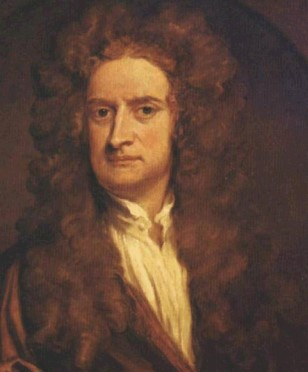
\includegraphics[width=\textwidth]{example.jpg}
\end{minipage}



\vfill



\begin{minipage}{\textwidth}
\large \faUniversity \quad \CJKfamily{heiti} 教育经历 \hfill EDUCATION\\
\rule[8pt]{\textwidth}{1pt}
\small
\normalfont
\begin{tabular}{m{0.2\textwidth}<{\raggedright}m{0.5\textwidth}<{\centering}m{0.25\textwidth}<{\centering}}
	1654-1661&金格斯皇家中学&XX专业\\
	1661-1665&剑桥大学,三一学院&XX专业\\
\end{tabular}

\vspace{1em}
\large \faUserGraduate \quad \CJKfamily{heiti} 个人情况 \hfill PERSONAL INFORMATION\\
\rule[8pt]{\textwidth}{1pt}
\small
\begin{tabular}{p{4em}<{\raggedright}p{0.88\textwidth}<{\raggedright}}
	研究方向&\normalfont 微积分学、光学、力学、哲学\\
	专业技能&\normalfont 引力及其对行星轨道的作用、开普勒的行星运动定律、与胡克和弗拉姆斯蒂德在力学上的讨论;物体运动的三个基本定律;牛顿与莱布尼茨独立发展出了微积分学,并为之创造了各自独特的符号;广义二项式定理,牛顿恒等式、牛顿法,立方面曲线(两变量的三次多项式);光的微粒说\\
	英语水平&\normalfont 英国人\\
\end{tabular}
\end{minipage}


\vfill


\begin{minipage}{\textwidth}
\large \faFile \quad \CJKfamily{heiti} 学术论文 \hfill PAPER LIST\\
\rule[8pt]{\textwidth}{1pt}
\small
\textbf{ACCEPTED:}\\
\textit{Philosophiae Naturalis Principia Mathematica}. Issac Newton. 1687.\\
\textit{Hypothesis Explaining the Properties of Light}. Issac Newton. 1675.\\
\textit{Optics}. Issac Newton. 1675.\\
\textbf{UNDER REVIEW:}\\
Paper. Author. Submitted to \emph{Journal or Conference}. \href{https://arxiv.org/abs/XXXX}{\textit{arXiv preprint} arXiv: XXXX}.\\
\end{minipage}




\vfill

\begin{minipage}{\textwidth}
\large \faClipboardList \quad \CJKfamily{heiti} 科研项目 \hfill RESEARCH PROJECT\\
\rule[8pt]{\textwidth}{1pt}
\small
\normalfont
在力学上,牛顿阐明了动量和角动量守恒的原理,提出牛顿运动定律。在光学上,他发明了反射望远镜,并基于对三棱镜将白光发散成可见光谱的观察,发展出了颜色理论。他还系统地表述了冷却定律,并研究了音速。\\
在数学上,牛顿与莱布尼茨分享了发展出微积分学的荣誉。他也证明了广义二项式定理,提出了“牛顿法”以趋近函数的零点,并为幂级数的研究做出了贡献。\\
在经济学上,牛顿提出金本位制度。\\
\end{minipage}


\vfill

\begin{minipage}{\textwidth}
\large \faClipboardList \quad \CJKfamily{heiti} 竞赛项目 \hfill COMPETITIONS\\
\rule[8pt]{\textwidth}{1pt}
\small
\normalfont

\begin{tabular}{m{0.3\textwidth}<{\raggedright}m{0.4\textwidth}<{\centering}m{0.3\textwidth}<{\centering}}
	竞赛内容&\href{https://大赛官网或项目链接}{竞赛标题}&获得奖项\\
	竞赛内容&\href{https://大赛官网或项目链接}{竞赛标题}&获得奖项\\
	竞赛内容&\href{https://大赛官网或项目链接}{竞赛标题}&获得奖项\\
\end{tabular}
\end{minipage}



\newpage

\huge \CJKfamily{heiti} 个人自述\hfill PERSONAL STATEMENT
\rule[20pt]{\linewidth}{1.5pt}

\normalsize\normalfont
\begin{spacing}{1.5}
\qquad 艾萨克·牛顿(1643年1月4日—1727年3月31日),爵士,英国皇家学会会长,英国著名的物理学家、数学家,百科全书式的“全才”,著有《自然哲学的数学原理》、《光学》。

\qquad 他在1687年发表的论文《自然定律》里,对万有引力和三大运动定律进行了描述。这些描述奠定了此后三个世纪里物理世界的科学观点,并成为了现代工程学的基础。他通过论证开普勒行星运动定律与他的引力理论间的一致性,展示了地面物体与天体的运动都遵循着相同的自然定律;为太阳中心说提供了强有力的理论支持,并推动了科学革命。

\qquad 在力学上,牛顿阐明了动量和角动量守恒的原理,提出牛顿运动定律。在光学上,他发明了反射望远镜,并基于对三棱镜将白光发散成可见光谱的观察,发展出了颜色理论。他还系统地表述了冷却定律,并研究了音速。

\qquad 在数学上,牛顿与戈特弗里德·威廉·莱布尼茨分享了发展出微积分学的荣誉。他也证明了广义二项式定理,提出了“牛顿法”以趋近函数的零点,并为幂级数的研究做出了贡献。在经济学上,牛顿提出金本位制度。
\end{spacing}








\end{document}